\documentclass[twocolumn, draft]{emulateapj}

\usepackage{amsmath}
\usepackage{graphics}
\usepackage{graphicx}
\usepackage{subfigure}
\usepackage{float}

\bibliographystyle{plainnat}

\begin{document}

\title{[Identification of Spectral Lines using Sparse Coding]}
\author{Andr\'es Riveros,
		Karim Pichara,
		Pavlos Protopapas,
		Diego Mardones,
		Paulina Troncoso and
		Mauricio Araya}

\begin{abstract}
Astronomy is facing new challenges on how to analyze big data and therefore, how to search or predict events/patterns of interest. The automatic detection and identification of spectral lines is an astronomical problem that has not been solved yet, so currently the identification is limited to the manual analysis of spectra by radio-astronomers. The use of spectroscopy allows to describe the chemical composition of astronomical objects through the emissions from the interaction between the radiation and the matter, thus causing emission lines. New observations in previously unexplored wavelength regions that will be available thanks to project as the Atacama Large Millimeter Array (ALMA), with which it is intended to use machine learning techniques to identify automatically these emission lines. Using simulated data based on the observations that has been obtained from the radio-telescope ALMA, it is proposed an algorithm with which to identify lines in order to determine the molecules that compose the observed galaxies. For this will be used the technique of Sparse Coding, that will evaluate the molecules that can origin the observed spectra, and it is expected to be found the best combination of molecules to recreate that spectra. From this algorithm, the astronomers may obtain a probability associated to the possible combinations of molecules composing astronomical objects.
\end{abstract}

\keywords{spectral lines: emission lines; spectroscophy techniques; method: data mining}

%%%%%%%%%%%%%%%%%%%%%%%%%%%%%%%%%%%%%%%%%%%%%%%%%%%%%%%%%%%%%%%%%%%%%%%%%%%%%%%
%%%%%%%%%%%%%%%%%%%%%%%%%%%%%%%%%%%%%%%%%%%%%%%%%%%%%%%%%%%%%%%%%%%%%%%%%%%%%%%
%%%%%%%%%%%%%%%%%%%%%%%%%%%%%%%%%%%%%%%%%%%%%%%%%%%%%%%%%%%%%%%%%%%%%%%%%%%%%%%
\section{Introduction}

This project is developed as part of a collaborative project between several Chilean universities for the initiative of the creation of the chilean virtual observatory Observatorio Virtual Chileno (ChiVO). ChiVO is an on-line platform that will make available to astronomers the measures of the radio-telescope Atacama Large Millimeter Array (ALMA). Also, ChiVO will provide several tools in order to process the data of ALMA measurements and to get specialized information of those measurements.

The data from the radio-telescope ALMA are of data cubes. The three dimensions correspond to two spatial dimension, and the third one of wave frequency. This means that for each spatial point can be obtained a spectrogram. The Pontifical Catholic University of Chile (PUC) will participate with the development of an algorithm to identify spectral lines using data mining techniques. This tool takes as input a observed spectra and returns a list with the best prediction of molecules that by the theoretical behavior their spectral lines describes the observed spectra.

Currently, there is not enough available ALMA data to train a model, so this project has been developed using synthetic data.
The Astronomical SYnthetic Data Observatory (ASYDO) project, a parallel project of ChiVO, will be the used in order to generate synthetic data to test the algorithm.

The objective of this investigation is to develop an algorithm that allows to identify spectral lines automatically in a simulated observed spectra. 
For this purpose, the objectives are the next:

The spectral lines must be codified into a convenient numerical representation in order to apply sparse coding techniques on them.

Must be determined the best possible collection of base spectra from the previous representation, in order to elaborate a dictionary.
The dictionary must be able to generate the most part of the simulated spectra data of ALMA.

Each combination of dictionary elements should give possible models of molecules that origin a spectra, so the combination of words of the dictionary represents a combinations of molecules that generates the spectra.

Finally, the combination that minimizes the error between the observed and generated spectra will be the combination of molecules predicted.

With this, the algorithm will be able to give as output the probabilities associated to the different possible combination of molecules that originated the observed spectra studied.

%%%%%%%%%%%%%%%%%%%%%%%%%%%%%%%%%%%%%%%%%%%%%%%%%%%%%%%%%%%%%%%%%%%%%%%%%%%%%%%
%%%%%%%%%%%%%%%%%%%%%%%%%%%%%%%%%%%%%%%%%%%%%%%%%%%%%%%%%%%%%%%%%%%%%%%%%%%%%%%
%%%%%%%%%%%%%%%%%%%%%%%%%%%%%%%%%%%%%%%%%%%%%%%%%%%%%%%%%%%%%%%%%%%%%%%%%%%%%%%
\section{Related work}
\label{sec:related}

The detection of spectral lines following the traditional method is limited to the manual analysis of the data in order to found the frequencies associated with the highest peaks in the spectral. Those peaks and a map with theoretical frequencies, and the experience of the astronomer, allow to classify those observations to certain molecules and its energies states.

The lack of scalability of this not automatized method, and the impractical mechanical process is not suitable for a big amount of data \citep{Schilke2001}. The difficulty of predicting new maps between the observed frequencies and the theoretical frequencies is given too by the blending of the lines. For those reasons, it would be desirable to automate this task.

El problema de mezclas de líneas y superposiciones son producto de tanto ruido como la falta de sensibilidad  para distinguir entre dos líneas en frecuencias cercanas. Lo anterior también puede producir peaks dobles en ciertas líneas \citep{Cernicharo2013}.

Un problema importante a la hora de identificar frecuencias subyace en líneas ópticamente delgadas, que tienden a dar resultados incorrectos. Usualmente, el uso de líneas de isotopos para su corrección resulta en un proceso costoso en tiempo y por lo mismo no es apto para datos masivos \citep{Schilke2001}.

Nummelin et al. \citep{Nummelin1998} propone el uso de un ajuste manual de las líneas a una forma arbitraria dada por una gausiana, obteniendo por cada línea su frecuencia observada, el peak en el brillo de temperatura y el ancho de la velocidad (ancho total a media altura), para así proceder con la identificación de la línea al asociarla con una molécula en cierto estado de energía. 

Para la identificación de líneas considerando las relaciones entre brillo de temperatura en un mismo espectro, es necesario asumir temperatura y origen homogéneo, dado que la diferencia de temperatura cambia la relación en serie de intensidades de líneas hiper-finas \citep{Nummelin2000}. 

Esto es importante a la hora de utilizar datos simulados con el fin de representar fielmente las características físicas de las estructuras a utilizar para entrenar, de modo que el modelo sea posteriormente aplicable sin mayores variaciones al utilizar datos reales de ALMA.

Es posible detectar patrones en las líneas que corresponden a la misma molécula e ispotropo a partir de intensidad relativa considerando que existe una razón entre diferencias de velocidad que es constante para un conjunto de líneas de emisión. Esto permite buscar patrones no tan solo de manera individual, sino que a través del análisis manual de series de líneas que se asocian a una misma molécula o átomo en sus diferentes estados energéticos. 

Los esfuerzos para desarrollar una herramienta automática de detección de líneas actualmente apuntan a herramientas semi-automáticas que utilizan como base complejos modelos físicos y químicos para la clasificación de líneas. 

XCLASS \footnote{\url{https://www.astro.uni-koeln.de/projects/schilke/XCLASS}}, 
CASSIS \footnote{\url{http://cassis.cesr.fr}} y 
WEEDS \footnote{\url{https://www.iram.fr/IRAMFR/GILDAS}} 
son herramientas que apuntan a modelar la composición de los espectros de tal forma que las simulaciones se asemejen a lo observado, existiendo grandes esfuerzos en realizar dichos modelamientos para solo la identificación de líneas. \citep{Schilke2011}.

Estas herramientas hacen uso de catálogos que contienen información sobre líneas espectroscópicas de moléculas y sus frecuencias teóricas de laboratorio, las que están disponibles públicamente en catálogos como (JPL \footnote{\url{http://spec.jpl.nasa.gov}}, 
CDMS \footnote{\url{http://www.astro.uni-koeln.de/cdms}}, 
Toyama \footnote{\url{http://www.sci.u-toyama.ac.jp/phys/4ken/atla}}) 
\citep{Schilke2011}, los que han sido compilados en 
Splatalogue \footnote{\url{http://www.splatalogue.net}} 
\citep{Remijan2008, Remijan2010}.

The above described techniques are not scalable to not rely on automated processes and analysis or manual adjustments with the imminent arrival of huge amounts of data from instruments such as ALMA, no longer apply. Therefore it is necessary to seek classification algorithms to delegate the task of identifying and classifying spectral lines.


%%%%%%%%%%%%%%%%%%%%%%%%%%%%%%%%%%%%%%%%%%%%%%%%%%%%%%%%%%%%%%%%%%%%%%%%%%%%%%%
%%%%%%%%%%%%%%%%%%%%%%%%%%%%%%%%%%%%%%%%%%%%%%%%%%%%%%%%%%%%%%%%%%%%%%%%%%%%%%%
%%%%%%%%%%%%%%%%%%%%%%%%%%%%%%%%%%%%%%%%%%%%%%%%%%%%%%%%%%%%%%%%%%%%%%%%%%%%%%%
\section{Background}
\label{sec:background}
%%%%%%%%%%%%%%%%%%%%%%%%%%%%%%%%%%%%%%%%%%%%%%%%%%%%%%%%%%%%%%%%%%%%%%%%%%%%%%%
\subsection{Sparse Coding}
%%%%%%%%%%%%%%%%%%%%%%%%%%%%%%%%%%%%%%%%%%%%%%%%%%%%%%%%%%%%%%%%%%%%%%%%%%%%%%%
\subsection{Spectroscopy}

Product of the radiation emitted by stellar objects, and its interaction with matter, emission lines are generated. This emission lines are distinctive for certain energy levels of molecules that make astronomical objects. The detection of emission lines and subsequent association with the molecules that cause them, about the structure of stellar objects.

The combination of these emission lines for each object allows a fingerprint of this unique, given its internal characteristics and different factors such as the temperature of the object, the speed with which it travels through space, etc.

With this information, it would have a large number of spectral lines, so arises the idea of ​​detecting these spectral lines as an astronomical problem of interest to apply data mining techniques.

On the side of data mining, there will be enough data to techniques and develop an algorithm for automatic identification. By astronomers, it may have a tool that automates the identification of emission lines in spectrograms belonging to astronomical objects.

Note that the objective of the algorithm is to support the rigor of a classification made by an expert, to serve as an initial preprocessing for this sort your lines, so it does not seek to completely replace the work of the expert, and is expected margin mistake for certain identifiable cases.

After defining the problem, need to establish a data set with which to begin developing the algorithm. Given the amount of spectrum needed to develop a predictive model, as currently do not have enough measurements of radio telescope, we chose to use a simulated spectra.


%%%%%%%%%%%%%%%%%%%%%%%%%%%%%%%%%%%%%%%%%%%%%%%%%%%%%%%%%%%%%%%%%%%%%%%%%%%%%%%
%%%%%%%%%%%%%%%%%%%%%%%%%%%%%%%%%%%%%%%%%%%%%%%%%%%%%%%%%%%%%%%%%%%%%%%%%%%%%%%
%%%%%%%%%%%%%%%%%%%%%%%%%%%%%%%%%%%%%%%%%%%%%%%%%%%%%%%%%%%%%%%%%%%%%%%%%%%%%%%
\section{Methodology}
\label{sec:methodology}

The methodology can be divided in several steps in order to find a solution for the problem:

\begin{description}
	\item [Identification of the problem] Identify the problem to solve: The scope of the problem and the type of data that will be used, in this case, the type of simulated ALMA data. Must be defined the parameters and subset of molecules to use.
	
	\item [Simulation of data] Especificaciones: Se deben definir con los parámetros de la simulación, así como un subconjunto de moléculas, en conjunto con astrónomos. Para esto deben considerarse las limitaciones de la simulación.
	
	\item [Related work] Se estudiará el estado del arte en la clasificación de líneas espectrales. Se buscarán situaciones similares con el fin de aplicar técnicas adecuadas a este caso. For the codification of the spectra in order to represent the presence of molecules in a observed spectra. To archive this, the previous related work like Raman spectroscopy (Howle, ett al. 2005) (O' Connell et all) can be useful. \citep{howley_effect_2005}.
	
	\item [Development of the solution] se realizará una iteración de soluciones al problema de codificación sparse, analizando el efecto de los parámetros en los modelos a utilizar y determinando la cantidad de parámetros necesarios para abarcar mayor complejidad en la identificación de los espectros. Optimize the solution of the sparse coding problem. Analize the effect of each parameter of the model.
	
\end{description}


\subsection{Splatalogue}

\begin{figure}[ht]
	\centering
	
\includegraphics[width=5cm]{figs/fig1.pdf}
	\caption{...}
	\label{fig:fig1}
\end{figure}

\begin{figure*}[ht]
	\centering
	\subfigure[Title 2.1.]{
		
\includegraphics[width=5cm]{figs/fig2-1.pdf}
		\label{subfig:fig2-1}
	}
	\subfigure[Title 2.2.]{
		
\includegraphics[width=5cm]{figs/fig2-2.pdf}
		\label{subfig:fig2-2}
	}
	\caption{In figure \ref{subfig:fig2-2} is shown that ...}
	\label{fig:subfigs}
\end{figure*}

%%%%%%%%%%%%%%%%%%%%%%%%%%%%%%%%%%%%%%%%%%%%%%%%%%%%%%%%%%%%%%%%%%%%%%%%%%%%%%%
\subsection{Synthetic Data}

To develop the algorithm for identifying spectral lines web service that provides simulated data goat is used. This project, called Astronomical Observatory Data synthetic (ASYDO) runs parallel to this project as part of the tools you can use to astronomers as web service. This project is available at
 \footnote\url{https://github.com/ChileanVirtualObservatory/ASYDO}.


The simulation will generate a set of training to develop the identification algorithm proposed in this project. As this service simulation an important input algorithm development, there have been a series of meetings to work together and get a set of simulated appropriate data.

With the help of astronomers involved in the goat project has been given the necessary parameters to perform the simulation. Defined the complexity and importance of replicating certain features that help you get curves that approach spectra enough data to be obtained from observations of ALMA.

For the algorithm developed is correctly simulated data, it should be included in the meta-data cubes emission lines present in the spectra. This will be possible to evaluate the predictive model and determine metrics to validate the predictions.

The characteristics of ALMA measurements have yielded the following specifications when simulating cubes ALMA data type:

\begin {table}[H]
\begin{center}
	\begin{tabular}{|c|c|}
		\hline Ancho de banda espectral & 4000 MHz \\ 
		\hline Resolusión espectral & 1 MHz \\ 
		\hline 
	\end{tabular}
	\caption {Common specifications for all simulated data cubes.}
\end{center}
\end{table}

And as input parameters, the user will need to provide:

\begin {table}[H]
\begin{center}
	\begin{tabular}{|c|c|}
		\hline Frecuencia central &  MHz \\ 
		\hline Resolusión espectral & 1 MHz \\ 
		\hline Asención &  Grados \\ 
		\hline Declinación & Grados \\ 
		\hline Ancho de las lineas & (fwhm) \\ 
		\hline 
	\end{tabular}
	\caption {Parameters provided by the user for data cubes simulated.}
\end{center}
\end{table}

To represent measurements manner close to reality, was chosen with the help of a set of molecules astronomers and their isotopes. The criterion was to select molecules with a structure that is not in excess complicated, so that not involve unnecessary complexity for the algorithm. In addition, this set of molecules should be representative of the molecules that users expect of astronomical objects. These are shown in the following table.

\begin {table}[H]
\begin{center}
	\begin{tabular}{|c|c|c|}
		\hline Nombre & Fórmula &  Isótopos \\ 
		
		\hline 	Carbon Monoxide & 'CO' & 'COv=0',\\
		&        &  'COv=1','13COv=0',\\
		&	   & 'C18O', 'C17O','13C17O', \\
		&	   & '13C18O'\\
		
		\hline	Diazenylium & 'N2H' & 'N2H+v=0',\\
		&        &   'N2D+', '15NNH+', 'N15NH+' \\
		
		\hline	Cyanide Radical & 'CN' & 'CNv=0', '13CN', 'C15N' \\
		
		\hline	Hydrogen Cyanide & 'HCN' & 'HCNv=0', 'HCNv2=1',\\
		&        &   'HCNv2=2','HCNv3=1' \\
		&       & 'HC15Nv=0', 'H13CNv2=1'\\
		&        &   'H13CNv=0'\\
		&       & 'HCNv1=1', 'HCNv3=1',\\
		&        &   'DCNv=0'\\
		&       & 'DCNv2=1', 'HCNv2=4',\\
		&        &    'HCNv2=1 1-v2=4 0' \\
		
		\hline  Carbon Monosulfide & 'CS' & 'CSv=0',\\
		&        &   '13C34Sv=0', 'C36Sv=0'\\
		&      & 'C34Sv=0', 'CSv=1-0',\\
		&        &   '13CSv=0'\\
		&      & 'C33Sv=0', 'CSv=1', 'C34Sv=1' \\
		
		\hline	Thioxoethenylidene & 'CCS' & 'CCS', 'C13CS',\\
		&        &   '13CCS', 'CC34S' \\
		
		\hline	Hydrogen sulfide & 'H2S' & 'H2S', 'H2S', 'H234S', 'D2S' \\
		
		\hline	Thioformaldehyde & 'H2CS' & 'H2CS', 'H213CS', 'H2C34S' \\
		
		\hline	Sulfur Dioxide & 'SO2' & 'SO2v=0', '33SO2',\\
		&        &   '34SO2v=0', 'SO2v2=1' \\
		
		\hline	Sulfur Dioxide & 'OSO' & 'OS18O', 'OS17O' \\
		
		\hline	Formaldehyde & 'H2CO'  & 'H2CO', 'H2C18O', 'H213CO' \\
		
		\hline	Formylium & 'HCO'  & 'HCO+v=0', 'HC18O+',\\
		 &        &  'HC17O+', 'H13CO+' \\
		
		
		\hline	Cyanobutadiyne & 'HC5N' & 'HC5Nv=0', 'HC5Nv11=1',\\
		&        &  'HCC13CCCN', 'HCCCC13CN'\\
		&        &  'HCCC13CCN', 'H13CCCCCN'\\
		&        & 'HC13CCCCN' \\
		
		\hline	Methanol & 'CH3OH' & 'CH3OHvt=0',\\
		&        &   '13CH3OHvt=0 ', 'CH318OH' \\
		&      & 'CH3OHvt=1 ', '13CH3OHvt=1'\\
		
		\hline 
	\end{tabular}
	\caption {Set of molecules and isotropic with which the simulations were performed.}
\end{center}
\end{table}


%%%%%%%%%%%%%%%%%%%%%%%%%%%%%%%%%%%%%%%%%%%%%%%%%%%%%%%%%%%%%%%%%%%%%%%%%%%%%%%
\subsection{Codification}

The proposed algorithm aims at identifying the molecular components that are part of different simulated astronomical objects. For this, we analyze the spectral lines from the spectra of these astronomical objects, in order to find patterns and predict its composition.

For an astronomical object, observe their spectral lines can help identify the molecules that compose it, since for each energy state of these molecules, being those present in the object, manifested in emission lines along their spectra observed at certain frequencies.

The algorithm takes advantage of this behavior and looks for patterns based on the presence of certain lines. When a molecule is present in the composition of an object, probably a number of lines should be observed along the spectrum. This means the fewer quee observed theoretical lines of said molecule, the lower the probability that the molecule forms part of the composition of the object.

So if there is confusion in identifying a spectroscopic line between two molecules, it is possible to perform a probabilistic prediction of the molecule to which corresponds the line based on the presence of each theoretical line along the spectrum being observed.


\subsection{Diseño del Prototipo}

Como se mencionó anteriormente, para el diseño del prototipo se utilizó el proyecto ASYDO. La temperatura en estas simulaciones no posee unidades, ya que las magnitudes de las líneas son relativas a la línea más alta de CO, a la cual se le ha asignado un valor arbitrariamente. Esto significa que los valores en sí mismos no poseen un significado.

El proceso para simular los cubos de prueba consistió en encontrar todas las moléculas y todos sus isotopos dentro de un rango de frecuencia. El rango de frecuencia utilizado para estas pruebas fue desde los 602000 MHz hasta los 606000 GHz, aproximadamente, que corresponde a la banda 9 de ALMA. Se corrió un script de líneas combinadas de varios subconjuntos aleatorios de isotopos, subconjunto de tamaño variable del total de moléculas teóricamente existentes en esta ventana de frecuencias utilizada.

El objetivo del algoritmo es entonces recuperar la lista de moléculas con la cual se generaron los cubos de datos. Para realizar esta tarea solo se pueden utilizar los espectrogramas observados. A través de métodos estadísticos se pretende predecir la presencia de ciertas moléculas y validar dichas predicciones al conocerse las moléculas utilizadas para generar las simulaciones.


\begin{figure}[H]
	\begin{center}
		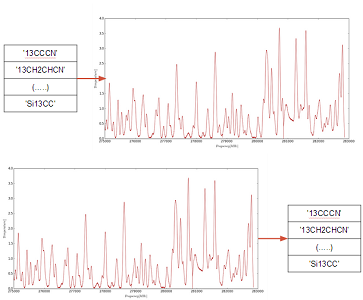
\includegraphics[width=70mm]{images/fig0}
		\caption{Se desea recuperar la lista de moléculas con la que se simuló el espectrograma. }
	\end{center}
\end{figure}



\subsection{Implementación}

El código de la implementación se encuentra disponible en el repositorio del proyecto de ChiVO en git. \footnote{\url{https://github.com/ChileanVirtualObservatory/DISPLAY}}

\subsubsection{Etapa de Detección}

El proceso de detección de líneas utiliza un parámetro de sensibilidad que determina si una medición es considerada una potencial línea espectroscópica. Esta sensibilidad depende de la desviación estándar del ruido en una región sin líneas visibles. Para obtener este parámetro se forzó a que en cada cubo, el pixel (0 , 0) no tuviese líneas espectrales, sino que solo ruido. Esto en la práctica se puede obtener seleccionando una región vacía del cubo de datos que el usuario previamente seleccione.

\begin{figure}[H]
	\begin{center}
		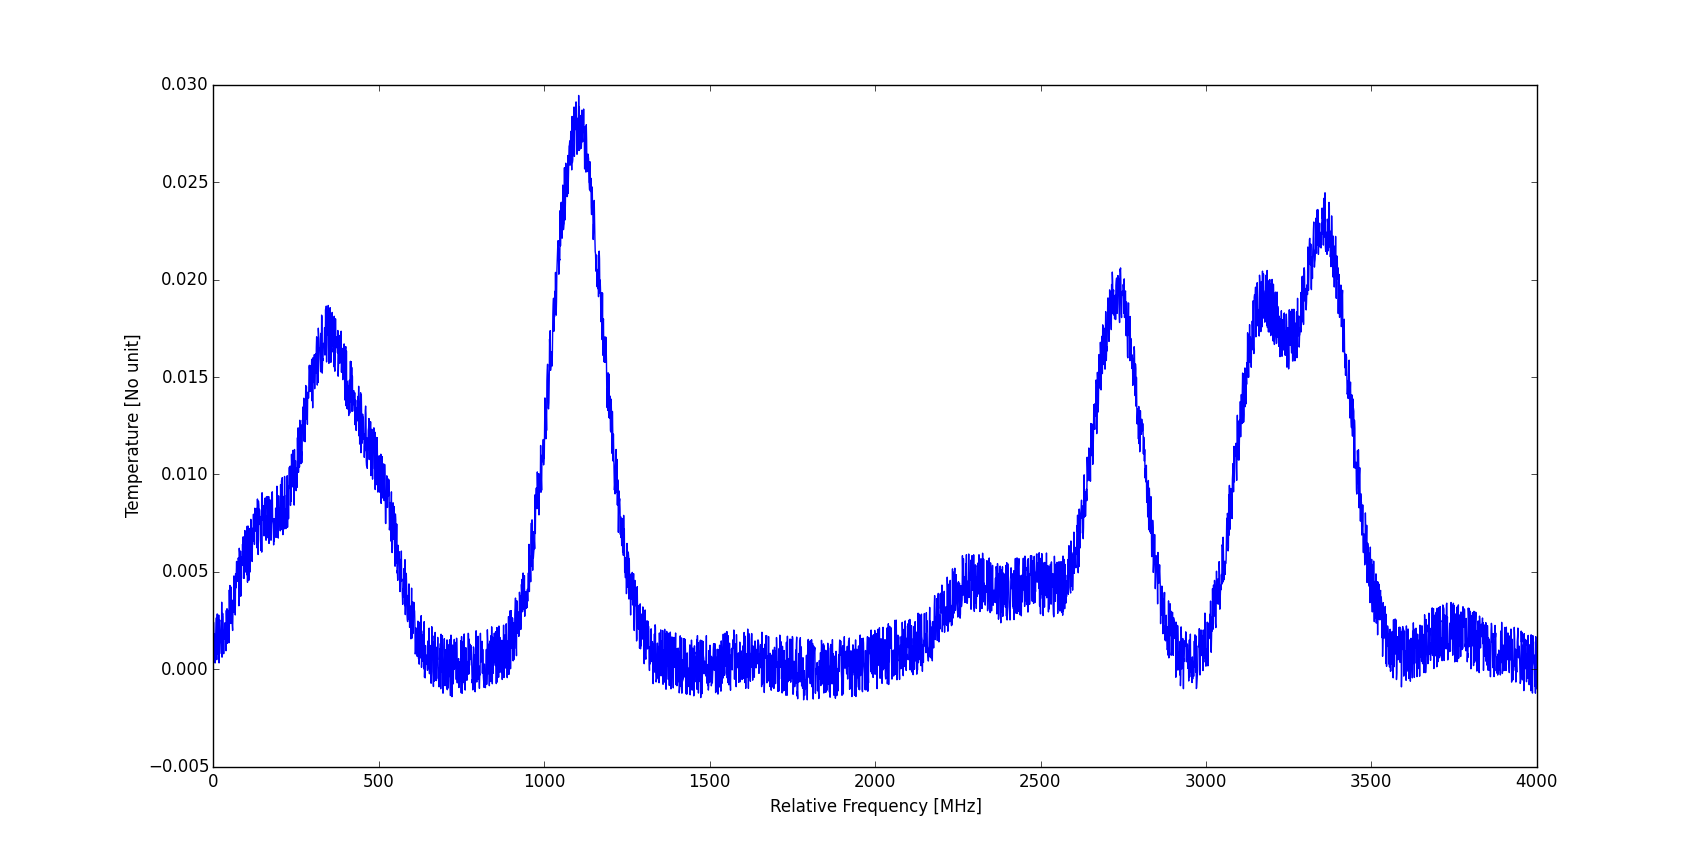
\includegraphics[width=70mm]{images/fig2}
		\caption{Espectro al situarse en un píxel espacial en particular. }
	\end{center}
\end{figure}

A continuación, para cada punto espacial del cubo de datos, se toma cada espectrograma de manera independiente. Lo primero es reducir el ruido de el espectro utilizando un filtro de Savitzky-Golay \citep{howley_effect_2005}. Este filtro utiliza un parámetro que indica el número de mediciones consecutivas a utilizar para suavizar la curva, por lo que el ancho de las curvas simuladas corresponde aun buen parámetro para ser asignado. Con este filtro se puede obtener un espectro con menor variación y así, identificar con mayor claridad las líneas. Este filtro se aplica al cubo completo, incluido el píxel con solo ruido, para hacer comparables los espectros al calcular la sensibilidad.

\begin{figure}[H]
	\begin{center}
		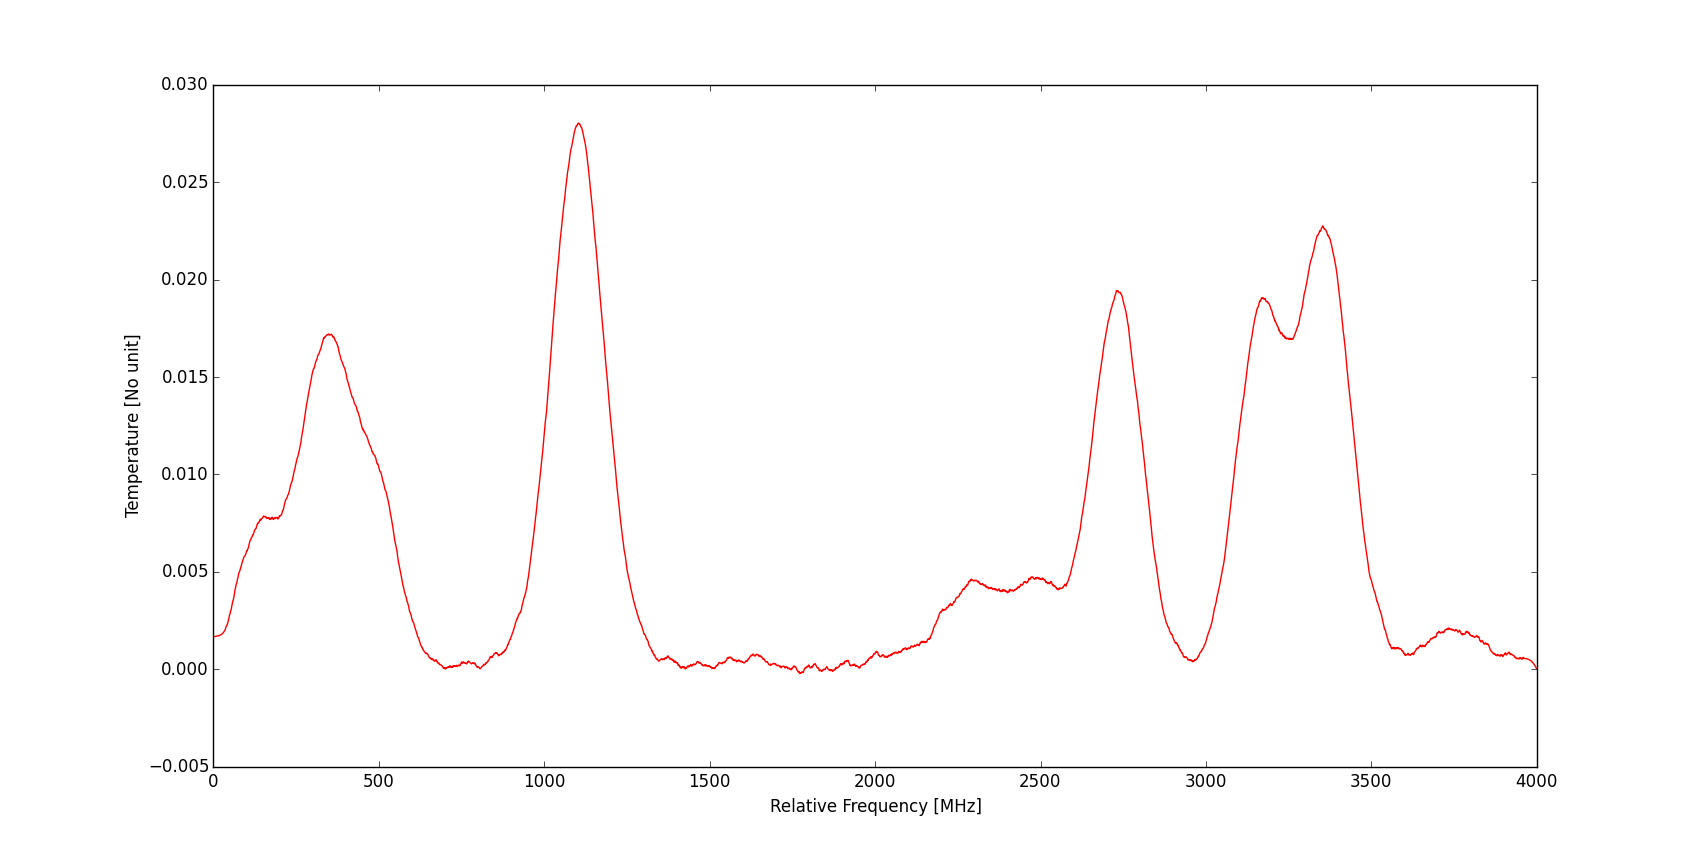
\includegraphics[width=70mm]{images/fig3}
		\caption{Espectro al reducir el ruido con un filtro de Savitzky-Golay. }
	\end{center}
\end{figure}


Se comienza con la determinación de los puntos máximos de la curva observada. Es posible asignar un parámetro que determina la distancia máxima que debe existir entre el brillo de dos frecuencias consecutivas para ser considerados un máximo. Sin este parámetro, la curva tendría una serie de falsos máximos y mínimos producto del ruido existente en las mediciones. Así, cada máximo local detectado que está por sobre el parámetro de sensibilidad es un candidato a línea de emisión.

\begin{figure}[H]
	\begin{center}
		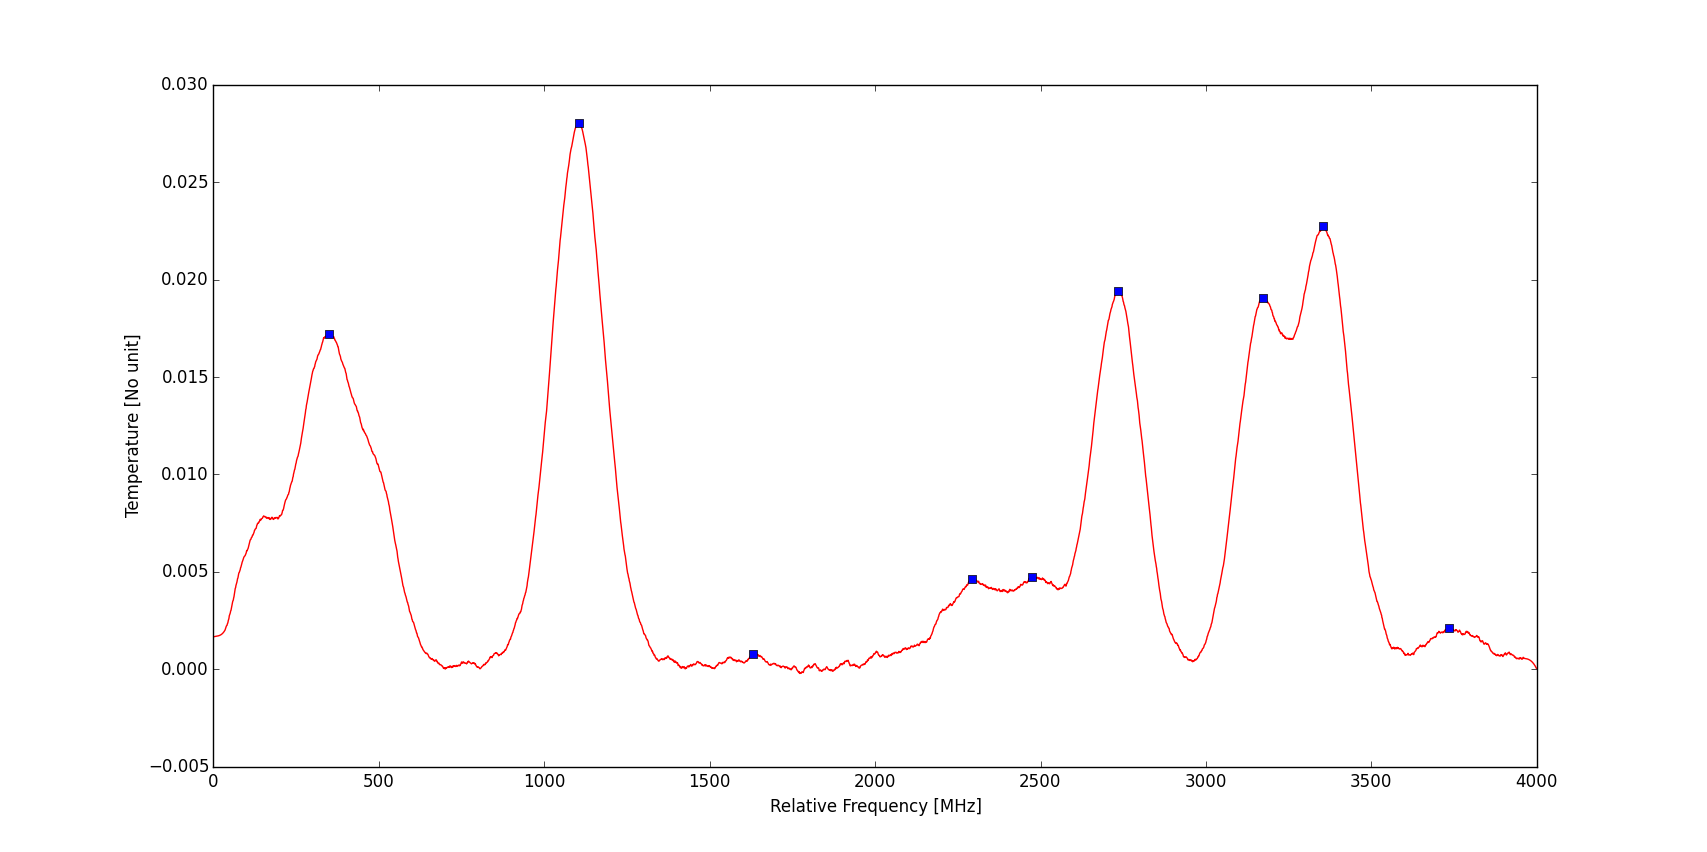
\includegraphics[width=70mm]{images/fig4}
		\caption{Puntos máximos locales por sobre el parámetro de sensibilidad. }
	\end{center}
\end{figure}

Al final del proceso, se crea un vector del tamaño del ancho de banda observado, donde se cada elemento del vector representa 1 Mhz del espectro. En cada frecuencia donde se detectó una línea, se asigna el valor 1, y cero en caso contrario.

\begin{figure}[H]
	\begin{center}
		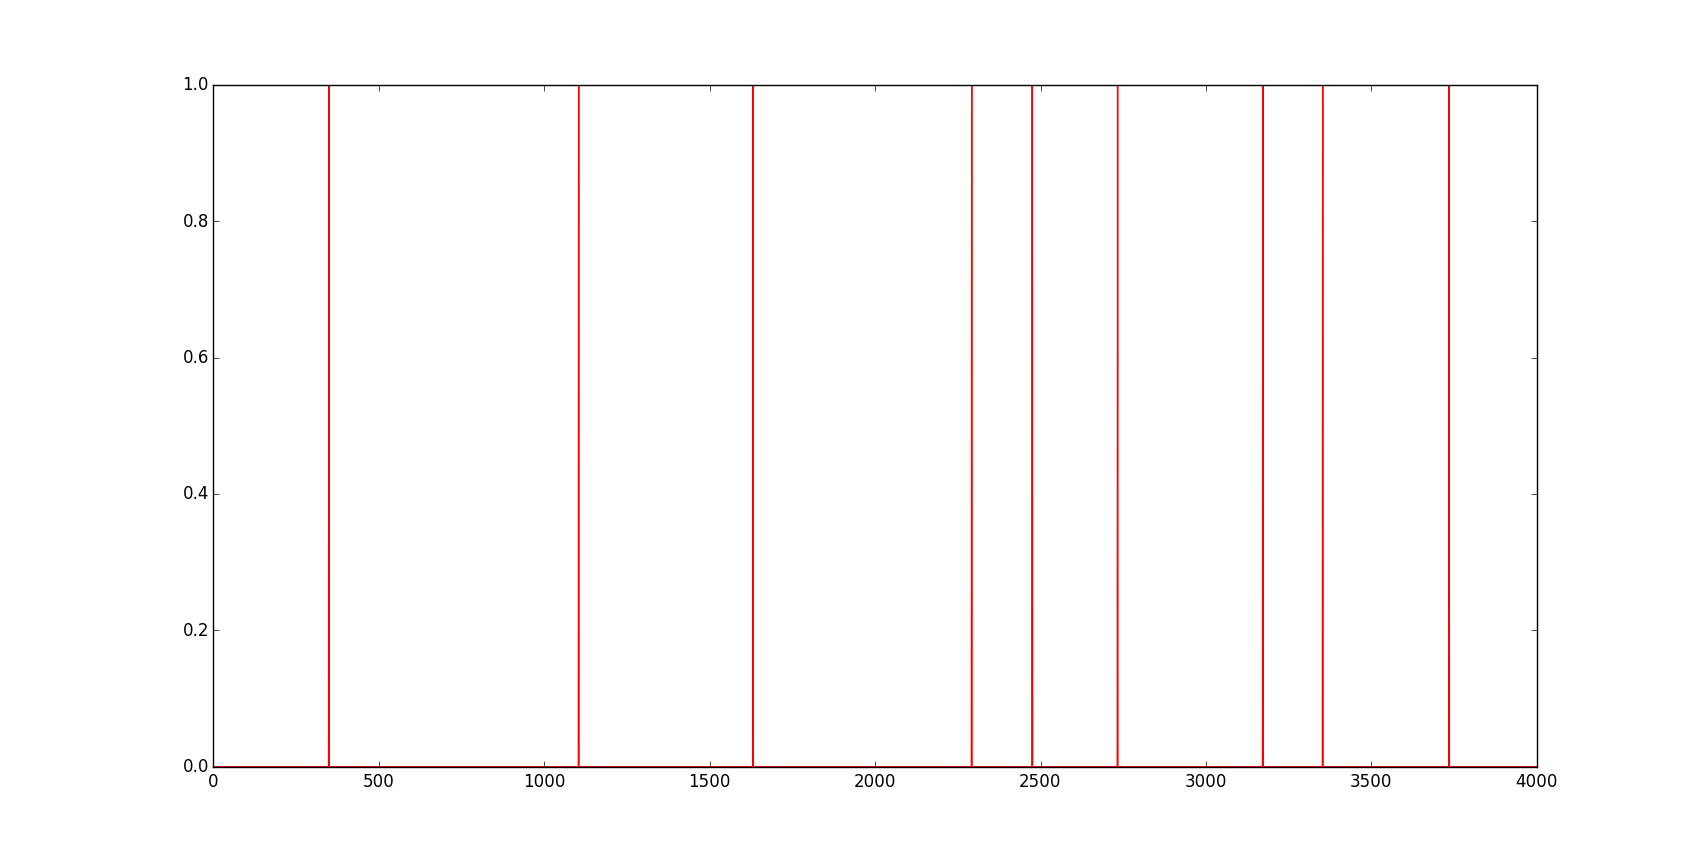
\includegraphics[width=70mm]{images/fig5}
		\caption{Gráfico del vector observado con valores no nulos en los puntos detectados. }
	\end{center}
\end{figure}

\begin {table}[H]
\begin{center}
	\begin{tabular}{|c|c|c|c|c|c|c|c|c|c|c|}
		\hline 0 & 0 &  ... &  1 & ... &  1 & ... & 1 & ... & 0 & 0 \\ 
		\hline
	\end{tabular}
	\caption {Forma del vector del espectro observado para el caso analizado.}
\end{center}
\end{table}

\subsubsection{Etapa de Predicción}

A continuación, se utiliza el catalogo de líneas espectroscópicas teóricas Splatalogue para obtener la lista de todas las frecuencias teóricas en el rango observado.

Para cada isotopo con líneas teóricas, se crea un vector del tamaño de la ventana en Mhz, similar al de la etapa de detección, donde el valor de cada posición es 1 si existe una línea teórica en dicha frecuencia para dicho isotopo, y cero en otro caso. Cada uno de estos vectores corresponde a una palabra de un diccionario de moléculas.

Posteriormente, se procesan las palabras de modo que solo tengan valores distintos de cero en las frecuencias donde el espectro observado es distinto de cero. Para esto, se asigna en dichas frecuencias la diferencia entre 1 y distancia exponencial entre la frecuencia observada y la frecuencia teórica más cercana, utilizando como parámetro sigma igual al ancho de las líneas espectrales.

Con esto se espera que las palabras que tienen frecuencias teóricas más cercanas a las observadas, tendrán valores mayores, con lo que el algoritmo de sparse coding tenga preferencia a elegir dichas palabras.

\begin{figure*}[ht]
	\centering
	\subfigure[Figura 6.1.]{
		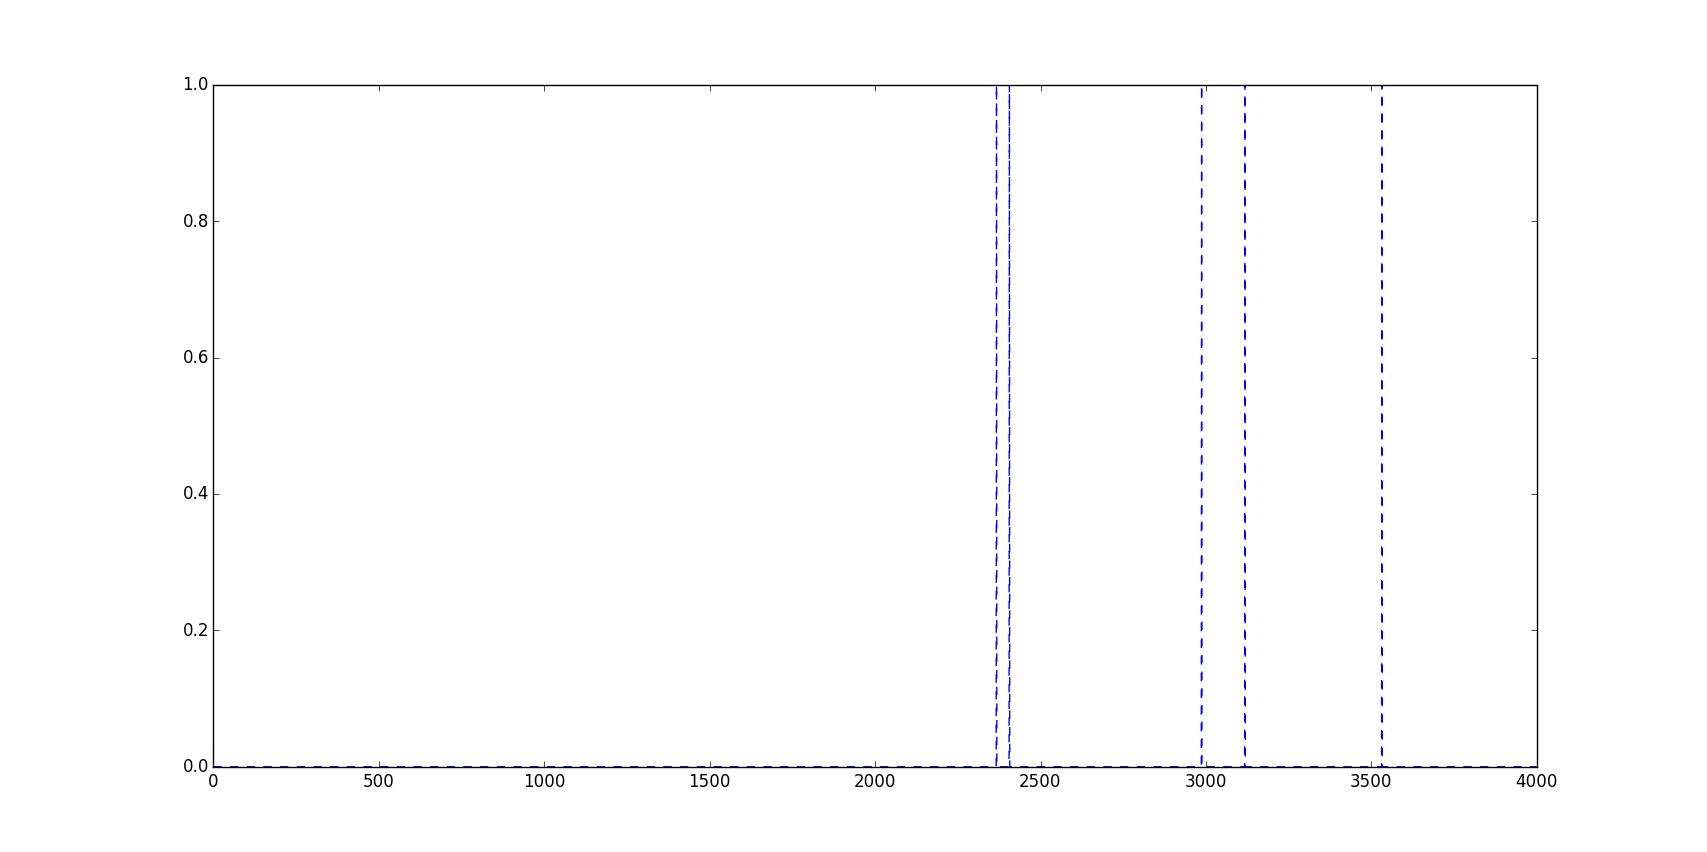
\includegraphics[width=100mm]{images/fig6-1}
		\label{subfig:fig6-1}
	}
	\subfigure[Figura 6.2.]{
		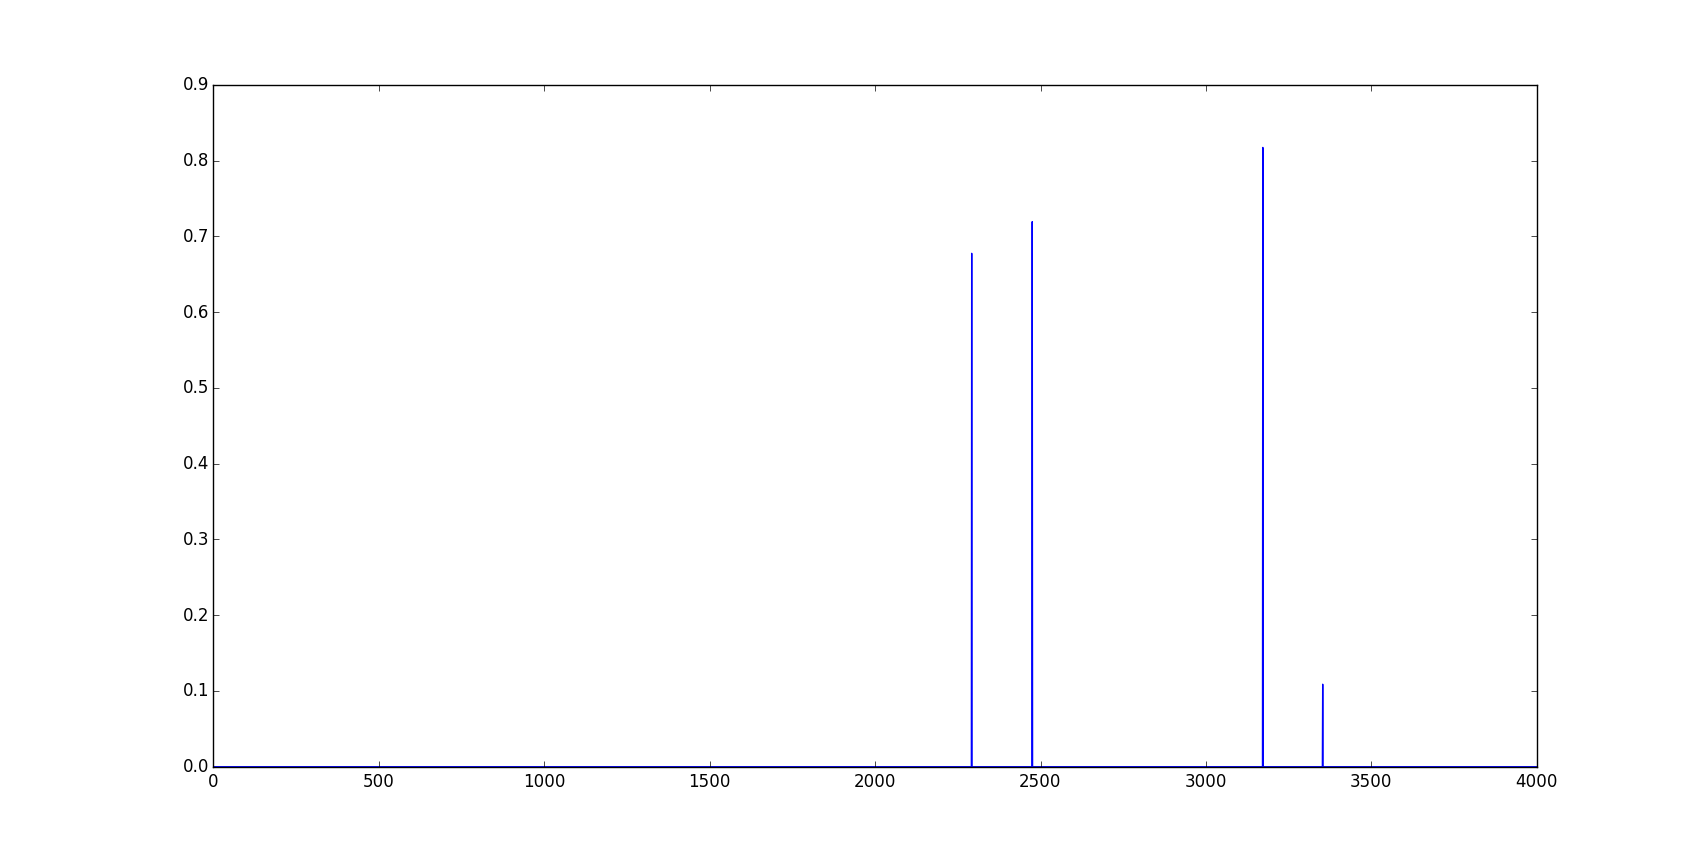
\includegraphics[width=100mm]{images/fig6-2}
		\label{subfig:fig6-2}
	}
	\caption{Rn la figura \ref{subfig:fig6-1} se grafica una palabra teórica y en la \ref{subfig:fig6-2} su equivalente recalculado}
\end{figure*}

La implementación se asegura de que cada frecuencia teórica cambie el valor de una y solo una frecuencia observada, y en caso de que haya otra frecuencia teórica que también tenga como frecuencia observada más cercana a la misma frecuencia, se asigna la menor distancia a dicha frecuencia observada. Con esto, cada palabra del diccionario queda con la misma o con menor cantidad de frecuencias distintas de cero.

\begin {table}[H]
\begin{center}
	\begin{tabular}{|c|c|c|c|c|c|c|c|c|c|c|c|}
		\hline Vector Obervado     & 0 & 0 &  0 &  1    & 0 &  1 & 0 & 1   & 0 & 0 & 0 \\ 
		\hline Palabra Teórica     & 0 & 0 &  1 &  0    & 0 &  1 & 0 & 0   & 0 & 0 & 1 \\ 
		\hline Palabra Recalculada & 0 & 0 &  0 &  0.88 & 0 &  1 & 0 & 0.6 & 0 & 0 & 0 \\ 
		\hline
	\end{tabular}
	\caption {Ejemplo de recálculo de una palabra utilizando para la distancia exponencial sigma = 2.}
\end{center}
\end{table}

Finalmente, se tiene un problema de optimización con una formulación de sparse coding, donde se intenta acercar  al máximo la combinación lineal entre palabras de tal forma que se construya el vector del espectro observado. El paramero de sparsity permite restringir la cantidad de palabras que se desea que el modelo utilice para formar la observación. En este caso se asignó un valor elevado para que el modelo pudiese acercarse lo máximo posible a la observación sin límite de palabras.  La función a minimizar en esta formulación es la norma l-2 y corresponde al error cuadrático medio.

%%%%%%%%%%%%%%%%%%%%%%%%%%%%%%%%%%%%%%%%%%%%%%%%%%%%%%%%%%%%%%%%%%%%%%%%%%%%%%%
%%%%%%%%%%%%%%%%%%%%%%%%%%%%%%%%%%%%%%%%%%%%%%%%%%%%%%%%%%%%%%%%%%%%%%%%%%%%%%%
%%%%%%%%%%%%%%%%%%%%%%%%%%%%%%%%%%%%%%%%%%%%%%%%%%%%%%%%%%%%%%%%%%%%%%%%%%%%%%%
\section{Results}
\label{sec:results}

\begin{center}
	$min_{\alpha} ||x-D\alpha||_2^2$ 
	$s.a.$ 
	$||\alpha||_1 \leq \lambda$ \\
	$x$ : vector observado, 
	$D$ : diccionario recalculado, 
	$\lambda$ : parámetro de spartity, 
	$||()||_2$ : Norma l-2
\end{center}


La solución óptima debería utilizar solo las palabras asociadas a los isotopos presentes en el espectro. En la siguiente tabla se puede ver la simulación realizada y los isotopos rescatados:

\begin {table}[H]
\begin{center}
	\begin{tabular}{|c|c|c|}
		\hline Nombre & Fórmula &  Isótopos \\ 
		
		
		\hline	Hydrogen Cyanide & 'HCN' & 'HC15Nv=0',\\
		&        &   'H13CNv2=1', 'H13CNv=0'\\ 
		
		\hline	Thioformaldehyde & 'H2CS' & 'H213CS' \\
		
		\hline	Sulfur Dioxide & 'SO2' & 'SO2v=0', 'SO2v2=1' \\
		
		\hline	Sulfur Dioxide & 'OSO' & 'OS18O', 'OS17O' \\
		
		\hline	Formaldehyde & 'H2CO'  & 'H2C18O', 'H213CO' \\
		
		\hline 
	\end{tabular}
	\caption {Conjunto de isótopos con los que se realizaron simuló la implementación.}
\end{center}
\end{table}

\begin {table}[H]
\begin{center}
	\begin{tabular}{|c|c|c|c|}
		\hline Nombre & Fórmula &  Isótopos & Alpha \\ 
		
		
		\hline	Hydrogen Cyanide & 'HCN'  & 'HC15Nv=0' & 0.0000\\
		&		  & 'H13CNv2=1' & 0.0000\\
		&		  & 'H13CNv=0' & 0.0000\\ 
		
		
		\hline	Thioformaldehyde & 'H2CS' & 'H213CS' & 0.0000\\
		
		\hline	Sulfur Dioxide & 'SO2'	  & 'SO2v=0' & 0.0000\\
		&		  & 'SO2v2=1'& 0.2694 \\
		
		\hline	Sulfur Dioxide & 'OSO' & 'OS18O' & 0.9612\\
		&	   & 'OS17O' & 0.5589\\
		
		\hline	Formaldehyde & 'H2CO'  & 'H2C18O' & 0.0000\\
		&		   & 'H213CO' & 0.0000\\
		
		\hline 
	\end{tabular}
	\caption {Set of isotopes in the simulation and is alphas.}
\end{center}
\end{table}

Cabe destacar que en este caso solo hubo un falso positivo, el isotopo '33SO2', con un valor de alpha de 0.6592. Esto significa que el algoritmo tiende a elegir los isotopos de moléculas con mayor cantidad de líneas en el ancho de banda observado, y es un aspecto a mejorar. 

Además, ciertas moléculas no son detectadas, y esto se puede deber a dos factores: en primer lugar, el algoritmo no logró detectarlas en la etapa anterior al no ser suficiente el filtro de ruido aplicado para que fuera identificada como máximo local o, en segundo lugar, no superó la sensibilidad dado que la variabilidad de la simulación hizo que no fuera observable. 

%\begin{figure}[H]
%	\begin{center}
%		
\includegraphics{images/fig1}
%		\caption{Espectro residual al sustraer una gausiana ajustada en una potencial línea de emisión. }
%	\end{center}
%\end{figure}

% Una forma de validación del algoritmo consiste en tomar un solo punto espacial del cubo como entrenamiento del algoritmo, y el resto de los pixeles como test de validación. De esta forma las palabras teóricas se recalcularán según las observaciones de dicho píxel espacial. En el resto de los píxeles del cubo, la variabilidad producto del effecto doppler interno y propia de la simulación  debería generar variaciones de forma que ciertas líneas se manifestarían y ciertas dejarían de observarse, a pesar de tener la misma composición.

% Si el algoritmo puede predecir los compuestos detectados en el píxel de referencia en el resto del cubo, se validaría esta aproximación al problema. De esta forma, se procedió a evaluar el algoritmo, obteniendo los siguientes resultados:

%%%%%%%%%%%%%%%%%%%%%%%%%%%%%%%%%%%%%%%%%%%%%%%%%%%%%%%%%%%%%%%%%%%%%%%%%%%%%%%
\subsection{Presence of Isotopes}

%%%%%%%%%%%%%%%%%%%%%%%%%%%%%%%%%%%%%%%%%%%%%%%%%%%%%%%%%%%%%%%%%%%%%%%%%%%%%%%
%%%%%%%%%%%%%%%%%%%%%%%%%%%%%%%%%%%%%%%%%%%%%%%%%%%%%%%%%%%%%%%%%%%%%%%%%%%%%%%
%%%%%%%%%%%%%%%%%%%%%%%%%%%%%%%%%%%%%%%%%%%%%%%%%%%%%%%%%%%%%%%%%%%%%%%%%%%%%%%
\section{Conclusions}
\label{sec:conclusions}

The sparse coding technique allows to identify much of the molecules, and even when it fails, the mismatch correspond to an isotope of the predicted molecule. With this, it is possible to give a basic notion of whick is the molecular composition of the astronomical objects simulated.

The data used to train the model did not included the high of the peaks observed in the spectra, given the limitation of the simulation. Those limitations reside in the inability to comply the theoretical relative heights of lines of the same isotope in a given spectra, assign the heights randomly.

This limitation was solved not using the height of the observed lines, but only the observed frequencies. So the solution consisted in the use of only the detected frequencies and assign for each isotope a value wich depends on the distance of the nearest theoretical frequency. Thus, the algorithm can relax the match between observed an theoretical frequencies.

The main difficulty of the current approach of this solution lies in that some molecules in some frequencies intervals are present with a large number of lines. As the words depends only on the observed frequency. Without consider the height, the importance of some observations is lost, besides it is a higher or a lower line, if it exist of it is just noise.

Therefore, an natural extension of this algorithm will be the incorporation of the height of the observed lines. With that information from future real data, will be possible to assign weights to avoid making this generalization of the importance of the observations. Also, one ratio between the relative heights of the lines of the same isotope help to have more representative words of reality.


%%%%%%%%%%%%%%%%%%%%%%%%%%%%%%%%%%%%%%%%%%%%%%%%%%%%%%%%%%%%%%%%%%%%%%%%%%%%%%%
%%%%%%%%%%%%%%%%%%%%%%%%%%%%%%%%%%%%%%%%%%%%%%%%%%%%%%%%%%%%%%%%%%%%%%%%%%%%%%%
%%%%%%%%%%%%%%%%%%%%%%%%%%%%%%%%%%%%%%%%%%%%%%%%%%%%%%%%%%%%%%%%%%%%%%%%%%%%%%%
\bibliography{paper-meta}

\end{document}
